\chapter{Node Beaconing Behavior}

Due to the fact that APRS is a source-routed protocol, most of the decisions as
to how often a station should send traffic and how far that traffic should
travel are allowed to be made by that originating station. 
The existing specification for the protocol hardly touches on this issue, 
while a great deal of time and energy is spent on the development forums 
bemoaning specific examples of misbehaving members of the network.
The two major parameters under the source node's control that are considered
here are the frequency of beaconing and the routing path used for each beacon.

Being a source-routed protocol does fundamentally introduces a
moral hazard in the network. For each node in the network to enjoy the
most benefit from the network, they would want to beacon as often as possible 
with the longest path allowed by the network.
It is only by mutual trust, respect, and education that this 
logic isn't universally followed and the network is not grossly oversubscribed
in the self-interest of every individual network node. 
Unfortunately, the most popular documentation on APRS fails to stress the 
importance of correctly configuring nodes in the best interest for the network
at large, and rarely gives any concrete guidance on what values should typically
be used when configuring various types of network nodes.


\section{Beaconing Algorithms}

For each APRS node with information available for the network,
a local decision needs to be made as to when that information will best 
serve the local network and should be transmitted. This is rarely a trivial 
decision, and one that could warrent much more creative and application or data
specific solutions than the ones presented here, which should be considered 
the typical minimum of most popular APRS trackers. The only datum considered 
in this paper is that of a mobile node's position, but these algorithms would
likely extend to most other user applications of APRS.

\subsection{Fixed Interval Beaconing}

The simplest beaconing algorithm consists of waiting a single fixed interval
between beacons, and only requires a single parameter that is the beacon interval.
When a tracker is turned on, it aquires a GPS lock and immediately sends out a 
beacon and starts a timer. Once that timer exceeds the beacon interval value, a 
new position is aquired from the GPS receiver and the new location is beaconed.
While simple, this algorithm does suffer from a number of inadequacies:
\begin{itemize}
\item The decision to beacon is made solely based on how long it has been
since the previous beacon, without considering any other information available
to the tracker. Examples of additional information would include whether the 
tracker has moved, how fast the tracker is moving, or any packets received from
the APRS network since the last beacon
\item A single fixed interval limits the amount of entropy introduced into the
network with regards to inter-packet arrival at other nodes. Since APRS is a 
CSMA shared channel network, it's tempting to use Poisson distribution models
for network capacity, which is likely invalid when the only source of entropy 
per tracker is the time when it was last turned on or gained GPS lock.
\end{itemize}

There are of course several possible extensions to the fixed interval beaconing
algorithm which each fix various deficiencies at the expense of simplicity.

\subsection{Time Slot Interval Beaconing}
\label{subsec:timeslot}

Arguably a more restrictive form of fixed interval beaconing, time slotting is 
based on the idea of preventing channel collisions by allocating each tracker
a fixed time slot in each interval for when they are allowed to transmit.
An infeasible solution for the national APRS network due to its scale and lack
of coordination, time slotting is often applied where unusually high levels of
coordination do exist, such as special events and insular networks.

Time slotting introduces a new parameter called the slot time, and depends on every
tracker using it having syncronized real time clocks, which is reasonable since most
GPS receivers provide real time to within typically 200ms of UTC 
as part of their position reports
\footnote{The 200ms uncertainty is a typical value due to the delivery of time over
an asyncronous 4800 baud serial port. Internally, GPS receivers must maintain 
their real time clocks to several orders of magnitude higher precision than this
to be even remotely useful, but this precision isn't needed for APRS time slotting}.

The slot time determines how many seconds after the beginning of each interval
a tracker should beacon. The beginning of each interval is defined by the top of
the UTC hour\footnote{Specifying to use UTC time is remarkably 
	important, since UTC and GPS time have currently diverged by 16 seconds due to
	only UTC including leap seconds. Most, but not all, GPS receivers correctly
	compensate for this variable offset and report correct UTC time in their
GPRMC sentences}, and intervals run successively for the remainder of the hour.
For example, a tracker configured to time slot with an interval of 550 seconds and
a time slot of 12 would beacon at the following times:
\begin{itemize}
\item 00:00:12
\item 00:09:22
\item 00:18:32
\item 00:27:42
\item 00:36:52
\item 00:46:02
\item 00:55:12
\item 01:00:12
\end{itemize}

This deterministic beaconing algorithm allows carefully designed networks to 
over-subscribe network throughput well beyond the levels expected from 
the national APRS channel with its stocastic access methods. 
On an insular network seperate from the national
network, it would be possible to set an aggresively short beacon interval and 
carefully space trackers such that no two beacons colide with each other. 
This would make it possible to accomplish service levels such as
every-minute position updates from several dozen tracked vehicles, 
at the expense that there is no allowance for any additional traffic 
on the RF channel, and the network would depend on manual 
assurance that every tracker is configured to use its proper time slot.

\subsection{Nice Interval Beaconing}

Nice beaconing is a behavioral extension to fixed interval beaconing 
where trackers consider whether a ``echo"
of a position beacon is heard back from any near-by digital repeaters.
Since digipeaters tend to have much higher power transmitters and better quality
antennas than mobile trackers, once a packet is successfully received by any 
digipeater, that packet is much more likely to be received by a much larger
fraction of the target audience than directly from the low-power tracker. 
Most implementations introduce a new parameter
called nice \cite[p.~38]{ot3manual}, 
which is the number of subsequent beacons to skip when a digipeater echo is heard.

\subsection{Dithered Interval Beaconing}

One of the popular traffic models used for ALOHA-based networks assumes
that traffic enters the network as a Poisson process. 
This assumption has a number of implications for the total channel capacity, 
as will be discussed in chapter \ref{chap:channelcapacity},
but an important note for tracker behavior is the fact that fixed interval
beaconing introduces no new entropy once a tracker is activated and beaconing.

\begin{figure}
	\centering
	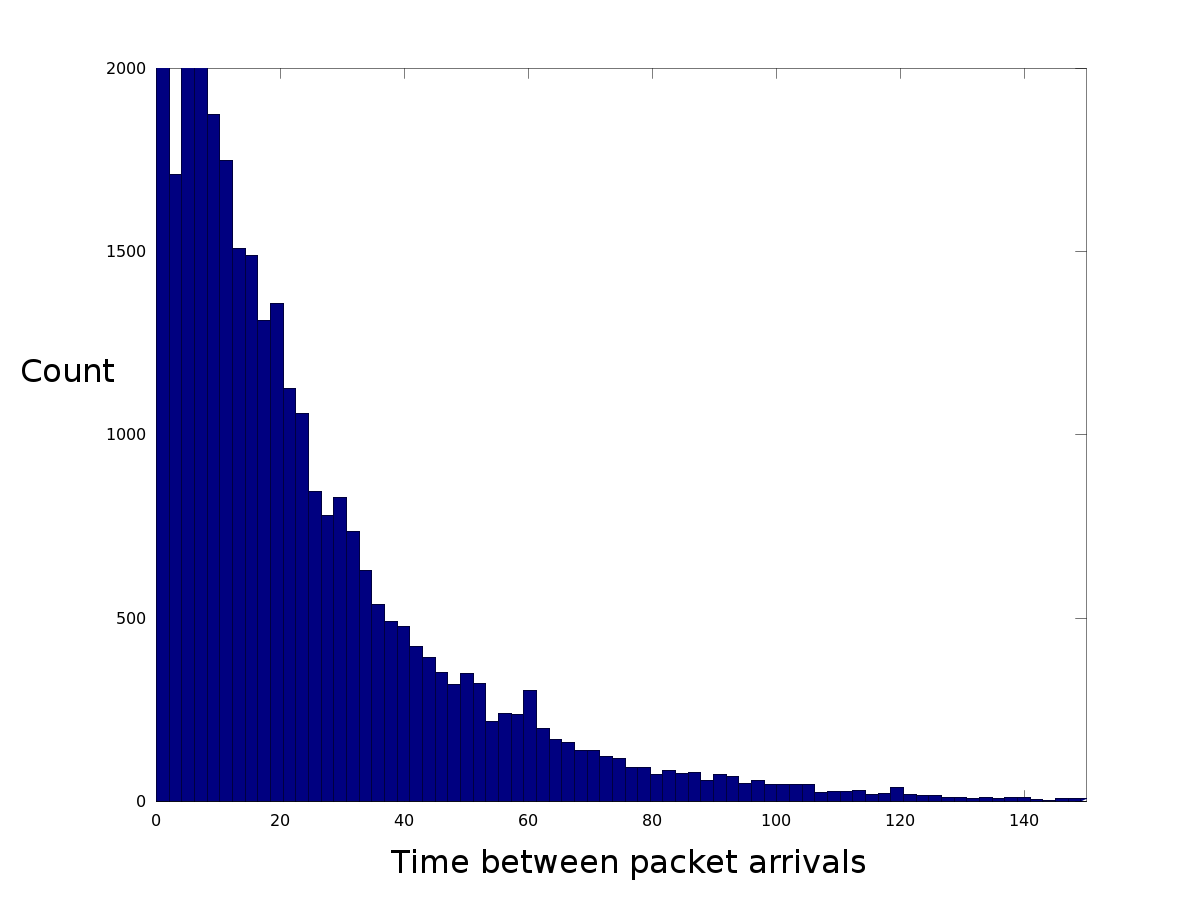
\includegraphics[width=0.7\textwidth]{src/slorfarrival}
	\caption{Packet arrival time spacing as measured over 10 days
	in San Luis Obispo, CA - TODO make better plot}
	\label{fig:rfarrivaldist}
\end{figure}

While there is no quantitative models measuring how far the current APRS 
network traffic deviates from a Poisson process, 
or how much this impacts network throughput,
observing the peaks at round numbers such as 60 and 120 second intervals
in plots such as figure \ref{fig:rfarrivaldist} indicate that the Poisson
assumption is not entirely valid.
Justifying the Poisson traffic model can be bolstered by trackers 
implementing what is called
dithering, where a small amount of noise is deliberately introduced on top
of the highly quantized beacon interval.

\begin{figure}
\begin{algorithmic}
\While {$beaconing$}
\State $interval\_delay \gets \Call{random}{ } \cdot beacon\_interval / 8$
	\State \Call{$sleep$}{$beacon\_interval + interval\_delay$}
	\State \Call{$send\_beacon$}{ }

\EndWhile
\end{algorithmic}
\caption{Beacon interval dithering algorithm}
\label{fig:ditheringalg}
\end{figure}

Developing analytical justifications for selecting specific distributions
are beyond the scope of this work, but it's theorized that introducing
any kind of entropy with approximately 1\% variance could improve network
traffic distribution.
Figure \ref{fig:ditheringalg} shows a possible implementation, where $RANDOM()$
is a function that returns a normalized distribution such as 
a uniform distribution in the range [0,1] 
or a Gaussian distribution with $\mu=0$ and $\sigma=1$.
The dividing factor of 8 was selected to scale the uniform distribution [0,1]
to yield a variance of 1\%, but that value was selected arbitrarily.

\subsection{SmartBeaconing}

SmartBeaconing\texttrademark is an adaptive beaconing algorithm developed
by Tony Arnerich and Steve Bragg for the HamHUD tracker kits \cite{smartbeacon}.
It allows trackers to make intelligent decisions as to how often to beacon
based on how ``interesting" the tracker's new position is. 
Vehicles moving in straight lines will tend to beacon at very long intervals,
but will beacon more often when making turns or traveling faster.
The algorithm is owned by HamHUD Nichetronix, LLC, and licensed freely
for non-commerical amateur radio applications.

This algorithm is particularly useful for APRS due to the fact that APRS
position reports support dead-reckoning, where they include a direction and 
velocity.
As long as trackers don't deviate from this advertised heading, there is
less reason to repeatedly beacon the tracker's new position.

The SmartBeaconing algorithm accepts up to seven parameters 
from the user\cite{smartbeaconwiki},
which are relatively more opaque than the one or two parameters required for
all the other popular interval algorithms. 
While there are suggested default values for each of these parameters, 
SmartBeaconing still proves to be controversial due to its users tending to
beacon much more often than 
trackers using other beaconing algorithms\cite{smartbeaconemail1}.
As discussed in chapter~\ref{chap:channelcapacity}, calculating the 
actual channel capacity in an area and the appropriate beaconing interval
for any of these algorithms are not at all straight forward.

\begin{itemize}
	\item low\_speed = 5 mph. This is the speed below which the tracker
		switches to the slow\_beacon\_interval 
		and no longer performs corner pegging.
	\item slow\_beacon\_interval = 1800 seconds. This is how often a tracker
		should beacon when it is moving slower than low\_speed, which indicates
		that it is essentially stopped.
	\item high\_speed = 60 mph. High speed is the value that slower speed
		beacon intervals are interpolated from. Speeds faster than high\_speed
		are valid but simply beacon at fast\_beacon\_interval.
	\item fast\_beacon\_interval = 180 seconds. This is how often a tracker should
		beacon when traveling at high\_speed and the scalar used to 
		calculate beacon intervals at lower speeds as a fraction of high\_speed.
	\item turn\_minimum = 30 degrees. The absolute minimum heading change needed 
		to trigger
		a ``corner peg" where the tracker beacons sooner than its speed warrants.
	\item turn\_slope = 255 degree miles per hour. 
		A scalar to convert between how fast a tracker is going and 
		how tight of a turn they need to perform to trigger a corner peg.
		The original documentation notes this value as unitless,
		which isn't entirely invalid since degree miles per hour isn't 
		a particularly helpful unit.
	\item turn\_beacon\_interval = 15 seconds. The maximum beacon rate allowed 
		when a tracker is changing heading often.
	
\end{itemize}

The original HamHUD algorithm is documented online as a snippet of C-like 
pseudocode as shown in figure~\ref{fig:hamhudsmartbeacon}.
In addition to the seven algorithm parameters, the pseudocode
requires the current speed and heading of the tracker, which are both
typically available from the \$GPRMC NMEA sentence \cite{nmearmc} provided by the 
tracker's GPS receiver, and the number of seconds since the last transmitted beacon.
Unfortunately, there are a number of issues with the provided code that
have possibly harmed deployment of the SmartBeaconing algorithm on other trackers:
\begin{itemize}
	\item Variable names change. Both ``speed" and ``mph" are used 
		to indicate the current speed of the tracker.
	\item Variable names are inconsistent. 
		slow\_rate is used for the beacon interval when the vehicle is stopped, 
		fast\_beacon\_rate for when the vehicle is moving,
		and turn\_time for when it is turning.
		A better set of variable names would be *\_beacon\_interval.
	\item The corner pegging algorithm suffers from an off-by-one error due to
		the final if statement being a $>$ comparison instead
		of a $\geq$ comparison. As documented, turning a corner would
		never cause an early beacon.
	\item The corner pegging section changes the value of secs\_since\_beacon
		instead of beacon\_rate, where secs\_since\_beacon is a system
		invariant that could possibly be implemented as a const
		or in-line function call.
	\item The SmartBeaconing documentation specifies that 
		the velocities used are in units
		of miles per hour, where velocities expressed in the APRS
		protocol are in knots.\footnote{APRS uses knots for velocity
			due to most GPS receivers outputting location
			data as NMEA 0183 sentences, which were originally designed 
			for maritime applications.}
\end{itemize}

Due to these issues, it seemed appropriate to rewrite the algorithm 
to correct these issues and to re-typeset the pseudocode in a more
contemporary style, which can be seen in figure~\ref{fig:kwfsmartbeacon}.

\begin{figure}[p]
\begin{lstlisting}
IF (speed < low_speed) {
	beacon_rate = slow_rate;
}
ELSE {
	// Adjust beacon rate according to speed
	IF (speed > high_speed) {
		beacon_rate = fast_beacon_rate;
	}
	ELSE {
		beacon_rate = fast_beacon_rate * high_speed / speed;
	}
	// Corner pegging - ALWAYS occurs if not "stopped"
	// Note turn threshold is speed-dependent
	turn_threshold = turn_min + turn_slope / mph;
	IF (heading_change_since_beacon > turn_threshold) AND
			(secs_since_beacon> turn_time) {
		secs_since_beacon = beacon_rate;
	}
}

IF (secs_since_beacon> beacon_rate)
	// ... send beacon
\end{lstlisting}
\caption{HamHUD SmartBeaconing Algorithm}
\label{fig:hamhudsmartbeacon}
\end{figure}

\begin{figure}[p]
\begin{algorithmic}
\If {$speed < low\_speed$}
	\State $beacon\_interval\gets slow\_beacon\_interval$

	%\Comment{Clamp slow speed beacon rate and skip corner pegging}
\Else
	\If {$speed > high\_speed$}
		\State $beacon\_interval\gets fast\_beacon\_interval$    

		%\Comment{Clamp high speed beacon rate}
	\Else
		\State $beacon\_interval\gets fast\_beacon\_interval \cdot high\_speed / speed$

		%\Comment{Interpolate beacon\_rate as a fraction of fast\_beacon\_rate}
	\EndIf


	\State $turn\_threshold\gets turn\_minimum + turn\_slope / speed$
	\If {$heading\_change\_since\_beacon > turn\_threshold$}
		\State $beacon\_interval\gets turn\_beacon\_interval$

		%\Comment{Corner pegging; threshold is speed dependent}
	\EndIf
\EndIf

\If {$secs\_since\_beacon \geq beacon\_interval$}
	\State \Call{$send\_beacon$}{ }

	%\Comment{Check if enough time has elapsed to send a new beacon}
\EndIf
\end{algorithmic}
\caption{Revised presentation of SmartBeaconing by the author}
\label{fig:kwfsmartbeacon}
\end{figure}


%\section{Path Recommendations}

%\begin{itemize}
%\item Fixed site: WIDE2-1 or literal Digis
%\item Mobile: WIDE1-1,WIDE2-1
%\item Airbore: No path
%\item Weather Stations: WIDE2-2?
%\item Proportional pathing
%\end{itemize}

